
%% bare_jrnl.tex
%% V1.4b
%% 2015/08/26
%% by Michael Shell
%% see http://www.michaelshell.org/
%% for current contact information.
%%
%% This is a skeleton file demonstrating the use of IEEEtran.cls
%% (requires IEEEtran.cls version 1.8b or later) with an IEEE
%% journal paper.
%%
%% Support sites:
%% http://www.michaelshell.org/tex/ieeetran/
%% http://www.ctan.org/pkg/ieeetran
%% and
%% http://www.ieee.org/

%%*************************************************************************
%% Legal Notice:
%% This code is offered as-is without any warranty either expressed or
%% implied; without even the implied warranty of MERCHANTABILITY or
%% FITNESS FOR A PARTICULAR PURPOSE! 
%% User assumes all risk.
%% In no event shall the IEEE or any contributor to this code be liable for
%% any damages or losses, including, but not limited to, incidental,
%% consequential, or any other damages, resulting from the use or misuse
%% of any information contained here.
%%
%% All comments are the opinions of their respective authors and are not
%% necessarily endorsed by the IEEE.
%%
%% This work is distributed under the LaTeX Project Public License (LPPL)
%% ( http://www.latex-project.org/ ) version 1.3, and may be freely used,
%% distributed and modified. A copy of the LPPL, version 1.3, is included
%% in the base LaTeX documentation of all distributions of LaTeX released
%% 2003/12/01 or later.
%% Retain all contribution notices and credits.
%% ** Modified files should be clearly indicated as such, including  **
%% ** renaming them and changing author support contact information. **
%%*************************************************************************


% *** Authors should verify (and, if needed, correct) their LaTeX system  ***
% *** with the testflow diagnostic prior to trusting their LaTeX platform ***
% *** with production work. The IEEE's font choices and paper sizes can   ***
% *** trigger bugs that do not appear when using other class files.       ***                          ***
% The testflow support page is at:
% http://www.michaelshell.org/tex/testflow/



\documentclass[journal]{IEEEtran}
%
% If IEEEtran.cls has not been installed into the LaTeX system files,
% manually specify the path to it like:
% \documentclass[journal]{../sty/IEEEtran}





% Some very useful LaTeX packages include:
% (uncomment the ones you want to load)


% *** MISC UTILITY PACKAGES ***
%
%\usepackage{ifpdf}
% Heiko Oberdiek's ifpdf.sty is very useful if you need conditional
% compilation based on whether the output is pdf or dvi.
% usage:
% \ifpdf
%   % pdf code
% \else
%   % dvi code
% \fi
% The latest version of ifpdf.sty can be obtained from:
% http://www.ctan.org/pkg/ifpdf
% Also, note that IEEEtran.cls V1.7 and later provides a builtin
% \ifCLASSINFOpdf conditional that works the same way.
% When switching from latex to pdflatex and vice-versa, the compiler may
% have to be run twice to clear warning/error messages.




% *** CITATION PACKAGES ***
%
%\usepackage{cite}
% cite.sty was written by Donald Arseneau
% V1.6 and later of IEEEtran pre-defines the format of the cite.sty package
% \cite{} output to follow that of the IEEE. Loading the cite package will
% result in citation numbers being automatically sorted and properly
% "compressed/ranged". e.g., [1], [9], [2], [7], [5], [6] without using
% cite.sty will become [1], [2], [5]--[7], [9] using cite.sty. cite.sty's
% \cite will automatically add leading space, if needed. Use cite.sty's
% noadjust option (cite.sty V3.8 and later) if you want to turn this off
% such as if a citation ever needs to be enclosed in parenthesis.
% cite.sty is already installed on most LaTeX systems. Be sure and use
% version 5.0 (2009-03-20) and later if using hyperref.sty.
% The latest version can be obtained at:
% http://www.ctan.org/pkg/cite
% The documentation is contained in the cite.sty file itself.






% *** GRAPHICS RELATED PACKAGES ***
%
\ifCLASSINFOpdf
  % \usepackage[pdftex]{graphicx}
  % declare the path(s) where your graphic files are
  % \graphicspath{{../pdf/}{../jpeg/}}
  % and their extensions so you won't have to specify these with
  % every instance of \includegraphics
  % \DeclareGraphicsExtensions{.pdf,.jpeg,.png}
\else
  % or other class option (dvipsone, dvipdf, if not using dvips). graphicx
  % will default to the driver specified in the system graphics.cfg if no
  % driver is specified.
  % \usepackage[dvips]{graphicx}
  % declare the path(s) where your graphic files are
  % \graphicspath{{../eps/}}
  % and their extensions so you won't have to specify these with
  % every instance of \includegraphics
  % \DeclareGraphicsExtensions{.eps}
\fi
% graphicx was written by David Carlisle and Sebastian Rahtz. It is
% required if you want graphics, photos, etc. graphicx.sty is already
% installed on most LaTeX systems. The latest version and documentation
% can be obtained at: 
% http://www.ctan.org/pkg/graphicx
% Another good source of documentation is "Using Imported Graphics in
% LaTeX2e" by Keith Reckdahl which can be found at:
% http://www.ctan.org/pkg/epslatex
%
% latex, and pdflatex in dvi mode, support graphics in encapsulated
% postscript (.eps) format. pdflatex in pdf mode supports graphics
% in .pdf, .jpeg, .png and .mps (metapost) formats. Users should ensure
% that all non-photo figures use a vector format (.eps, .pdf, .mps) and
% not a bitmapped formats (.jpeg, .png). The IEEE frowns on bitmapped formats
% which can result in "jaggedy"/blurry rendering of lines and letters as
% well as large increases in file sizes.
%
% You can find documentation about the pdfTeX application at:
% http://www.tug.org/applications/pdftex





% *** MATH PACKAGES ***
%
%\usepackage{amsmath}
% A popular package from the American Mathematical Society that provides
% many useful and powerful commands for dealing with mathematics.
%
% Note that the amsmath package sets \interdisplaylinepenalty to 10000
% thus preventing page breaks from occurring within multiline equations. Use:
%\interdisplaylinepenalty=2500
% after loading amsmath to restore such page breaks as IEEEtran.cls normally
% does. amsmath.sty is already installed on most LaTeX systems. The latest
% version and documentation can be obtained at:
% http://www.ctan.org/pkg/amsmath





% *** SPECIALIZED LIST PACKAGES ***
%
%\usepackage{algorithmic}
% algorithmic.sty was written by Peter Williams and Rogerio Brito.
% This package provides an algorithmic environment fo describing algorithms.
% You can use the algorithmic environment in-text or within a figure
% environment to provide for a floating algorithm. Do NOT use the algorithm
% floating environment provided by algorithm.sty (by the same authors) or
% algorithm2e.sty (by Christophe Fiorio) as the IEEE does not use dedicated
% algorithm float types and packages that provide these will not provide
% correct IEEE style captions. The latest version and documentation of
% algorithmic.sty can be obtained at:
% http://www.ctan.org/pkg/algorithms
% Also of interest may be the (relatively newer and more customizable)
% algorithmicx.sty package by Szasz Janos:
% http://www.ctan.org/pkg/algorithmicx




% *** ALIGNMENT PACKAGES ***
%
%\usepackage{array}
% Frank Mittelbach's and David Carlisle's array.sty patches and improves
% the standard LaTeX2e array and tabular environments to provide better
% appearance and additional user controls. As the default LaTeX2e table
% generation code is lacking to the point of almost being broken with
% respect to the quality of the end results, all users are strongly
% advised to use an enhanced (at the very least that provided by array.sty)
% set of table tools. array.sty is already installed on most systems. The
% latest version and documentation can be obtained at:
% http://www.ctan.org/pkg/array


% IEEEtran contains the IEEEeqnarray family of commands that can be used to
% generate multiline equations as well as matrices, tables, etc., of high
% quality.




% *** SUBFIGURE PACKAGES ***
%\ifCLASSOPTIONcompsoc
%  \usepackage[caption=false,font=normalsize,labelfont=sf,textfont=sf]{subfig}
%\else
%  \usepackage[caption=false,font=footnotesize]{subfig}
%\fi
% subfig.sty, written by Steven Douglas Cochran, is the modern replacement
% for subfigure.sty, the latter of which is no longer maintained and is
% incompatible with some LaTeX packages including fixltx2e. However,
% subfig.sty requires and automatically loads Axel Sommerfeldt's caption.sty
% which will override IEEEtran.cls' handling of captions and this will result
% in non-IEEE style figure/table captions. To prevent this problem, be sure
% and invoke subfig.sty's "caption=false" package option (available since
% subfig.sty version 1.3, 2005/06/28) as this is will preserve IEEEtran.cls
% handling of captions.
% Note that the Computer Society format requires a larger sans serif font
% than the serif footnote size font used in traditional IEEE formatting
% and thus the need to invoke different subfig.sty package options depending
% on whether compsoc mode has been enabled.
%
% The latest version and documentation of subfig.sty can be obtained at:
% http://www.ctan.org/pkg/subfig




% *** FLOAT PACKAGES ***
%
%\usepackage{fixltx2e}
% fixltx2e, the successor to the earlier fix2col.sty, was written by
% Frank Mittelbach and David Carlisle. This package corrects a few problems
% in the LaTeX2e kernel, the most notable of which is that in current
% LaTeX2e releases, the ordering of single and double column floats is not
% guaranteed to be preserved. Thus, an unpatched LaTeX2e can allow a
% single column figure to be placed prior to an earlier double column
% figure.
% Be aware that LaTeX2e kernels dated 2015 and later have fixltx2e.sty's
% corrections already built into the system in which case a warning will
% be issued if an attempt is made to load fixltx2e.sty as it is no longer
% needed.
% The latest version and documentation can be found at:
% http://www.ctan.org/pkg/fixltx2e


%\usepackage{stfloats}
% stfloats.sty was written by Sigitas Tolusis. This package gives LaTeX2e
% the ability to do double column floats at the bottom of the page as well
% as the top. (e.g., "\begin{figure*}[!b]" is not normally possible in
% LaTeX2e). It also provides a command:
%\fnbelowfloat
% to enable the placement of footnotes below bottom floats (the standard
% LaTeX2e kernel puts them above bottom floats). This is an invasive package
% which rewrites many portions of the LaTeX2e float routines. It may not work
% with other packages that modify the LaTeX2e float routines. The latest
% version and documentation can be obtained at:
% http://www.ctan.org/pkg/stfloats
% Do not use the stfloats baselinefloat ability as the IEEE does not allow
% \baselineskip to stretch. Authors submitting work to the IEEE should note
% that the IEEE rarely uses double column equations and that authors should try
% to avoid such use. Do not be tempted to use the cuted.sty or midfloat.sty
% packages (also by Sigitas Tolusis) as the IEEE does not format its papers in
% such ways.
% Do not attempt to use stfloats with fixltx2e as they are incompatible.
% Instead, use Morten Hogholm'a dblfloatfix which combines the features
% of both fixltx2e and stfloats:
%
% \usepackage{dblfloatfix}
% The latest version can be found at:
% http://www.ctan.org/pkg/dblfloatfix




%\ifCLASSOPTIONcaptionsoff
%  \usepackage[nomarkers]{endfloat}
% \let\MYoriglatexcaption\caption
% \renewcommand{\caption}[2][\relax]{\MYoriglatexcaption[#2]{#2}}
%\fi
% endfloat.sty was written by James Darrell McCauley, Jeff Goldberg and 
% Axel Sommerfeldt. This package may be useful when used in conjunction with 
% IEEEtran.cls'  captionsoff option. Some IEEE journals/societies require that
% submissions have lists of figures/tables at the end of the paper and that
% figures/tables without any captions are placed on a page by themselves at
% the end of the document. If needed, the draftcls IEEEtran class option or
% \CLASSINPUTbaselinestretch interface can be used to increase the line
% spacing as well. Be sure and use the nomarkers option of endfloat to
% prevent endfloat from "marking" where the figures would have been placed
% in the text. The two hack lines of code above are a slight modification of
% that suggested by in the endfloat docs (section 8.4.1) to ensure that
% the full captions always appear in the list of figures/tables - even if
% the user used the short optional argument of \caption[]{}.
% IEEE papers do not typically make use of \caption[]'s optional argument,
% so this should not be an issue. A similar trick can be used to disable
% captions of packages such as subfig.sty that lack options to turn off
% the subcaptions:
% For subfig.sty:
% \let\MYorigsubfloat\subfloat
% \renewcommand{\subfloat}[2][\relax]{\MYorigsubfloat[]{#2}}
% However, the above trick will not work if both optional arguments of
% the \subfloat command are used. Furthermore, there needs to be a
% description of each subfigure *somewhere* and endfloat does not add
% subfigure captions to its list of figures. Thus, the best approach is to
% avoid the use of subfigure captions (many IEEE journals avoid them anyway)
% and instead reference/explain all the subfigures within the main caption.
% The latest version of endfloat.sty and its documentation can obtained at:
% http://www.ctan.org/pkg/endfloat
%
% The IEEEtran \ifCLASSOPTIONcaptionsoff conditional can also be used
% later in the document, say, to conditionally put the References on a 
% page by themselves.




% *** PDF, URL AND HYPERLINK PACKAGES ***
%
%\usepackage{url}
% url.sty was written by Donald Arseneau. It provides better support for
% handling and breaking URLs. url.sty is already installed on most LaTeX
% systems. The latest version and documentation can be obtained at:
% http://www.ctan.org/pkg/url
% Basically, \url{my_url_here}.
\usepackage{float}
\usepackage{graphicx}



% *** Do not adjust lengths that control margins, column widths, etc. ***
% *** Do not use packages that alter fonts (such as pslatex).         ***
% There should be no need to do such things with IEEEtran.cls V1.6 and later.
% (Unless specifically asked to do so by the journal or conference you plan
% to submit to, of course. )


% correct bad hyphenation here
\hyphenation{op-tical net-works semi-conduc-tor}


\begin{document}
%
% paper title
% Titles are generally capitalized except for words such as a, an, and, as,
% at, but, by, for, in, nor, of, on, or, the, to and up, which are usually
% not capitalized unless they are the first or last word of the title.
% Linebreaks \\ can be used within to get better formatting as desired.
% Do not put math or special symbols in the title.
\title{Bare Demo of IEEEtran.cls\\ for IEEE Journals}
%
%
% author names and IEEE memberships
% note positions of commas and nonbreaking spaces ( ~ ) LaTeX will not break
% a structure at a ~ so this keeps an author's name from being broken across
% two lines.
% use \thanks{} to gain access to the first footnote area
% a separate \thanks must be used for each paragraph as LaTeX2e's \thanks
% was not built to handle multiple paragraphs
%

\author{Michael~Shell,~\IEEEmembership{Member,~IEEE,}
        John~Doe,~\IEEEmembership{Fellow,~OSA,}
        and~Jane~Doe,~\IEEEmembership{Life~Fellow,~IEEE}% <-this % stops a space
\thanks{M. Shell was with the Department
of Electrical and Computer Engineering, Georgia Institute of Technology, Atlanta,
GA, 30332 USA e-mail: (see http://www.michaelshell.org/contact.html).}% <-this % stops a space
\thanks{J. Doe and J. Doe are with Anonymous University.}% <-this % stops a space
\thanks{Manuscript received April 19, 2005; revised August 26, 2015.}}

% note the % following the last \IEEEmembership and also \thanks - 
% these prevent an unwanted space from occurring between the last author name
% and the end of the author line. i.e., if you had this:
% 
% \author{....lastname \thanks{...} \thanks{...} }
%                     ^------------^------------^----Do not want these spaces!
%
% a space would be appended to the last name and could cause every name on that
% line to be shifted left slightly. This is one of those "LaTeX things". For
% instance, "\textbf{A} \textbf{B}" will typeset as "A B" not "AB". To get
% "AB" then you have to do: "\textbf{A}\textbf{B}"
% \thanks is no different in this regard, so shield the last } of each \thanks
% that ends a line with a % and do not let a space in before the next \thanks.
% Spaces after \IEEEmembership other than the last one are OK (and needed) as
% you are supposed to have spaces between the names. For what it is worth,
% this is a minor point as most people would not even notice if the said evil
% space somehow managed to creep in.



% The paper headers
\markboth{Journal of \LaTeX\ Class Files,~Vol.~14, No.~8, August~2015}%
{Shell \MakeLowercase{\textit{et al.}}: Bare Demo of IEEEtran.cls for IEEE Journals}
% The only time the second header will appear is for the odd numbered pages
% after the title page when using the twoside option.
% 
% *** Note that you probably will NOT want to include the author's ***
% *** name in the headers of peer review papers.                   ***
% You can use \ifCLASSOPTIONpeerreview for conditional compilation here if
% you desire.




% If you want to put a publisher's ID mark on the page you can do it like
% this:
%\IEEEpubid{0000--0000/00\$00.00~\copyright~2015 IEEE}
% Remember, if you use this you must call \IEEEpubidadjcol in the second
% column for its text to clear the IEEEpubid mark.



% use for special paper notices
%\IEEEspecialpapernotice{(Invited Paper)}



% make the title area
\maketitle

% As a general rule, do not put math, special symbols or citations
% in the abstract or keywords.
\begin{abstract}
  Este relatório introduz a arquitetura de um \textit{Web Service} assim como seus componentes, o mesmo relata como foi implementado um Web Server que possui uma página web e serviços para busca de cidade e bairro através do CEP e rastreamento de encomendas dos correios.
\end{abstract}

% Note that keywords are not normally used for peerreview papers.
\begin{IEEEkeywords}
IEEE, IEEEtran, journal, \LaTeX, paper, template.
\end{IEEEkeywords}


\section{Introdução}
Com a disseminação de dispositivos com conexão a Internet na sociedade atual, houvesse a necessidade de criar/gerenciar serviços web, estes necessarios para atender as mais diversas funções como exemplo, salas de bate-papo, e-commerces e serviços meteorológicos entre outros.

Este relatório apresenta brevemente a arquitetura de um \textit{Web Service} e como foi implementado, serviços de consulta de cidade e barrio através do CEP e rastreamento de encomendas dos correios, juntamente com uma página web e um aplicativo androido que oferece uma interface para os serviços disponíveis.

O código deste relatório está em sua totalidade no endereço http://github.com/rafaelgov95/SD/Projeto-Correios-CEP, e o mesmo pode ser reutilizado sobre a licença MIT.
\section{Web Service}
Webservice é uma solução utilizada na integração de sistemas e na comunicação entre aplicações diferentes, como pode ser objservado na figura \ref{wbs}, um \textit{Data Server}, disponibiliza serviços para os mais diversos tipos de dispositivos, em diferentes formatos de objetos.

Com está tecnologia é possível que novas aplicações possam interagir com aquelas que já existem e que sistemas desenvolvidos em plataformas diferentes sejam compatíveis. 
\cite{webservece}.
\begin{figure}[H]
	\centering
	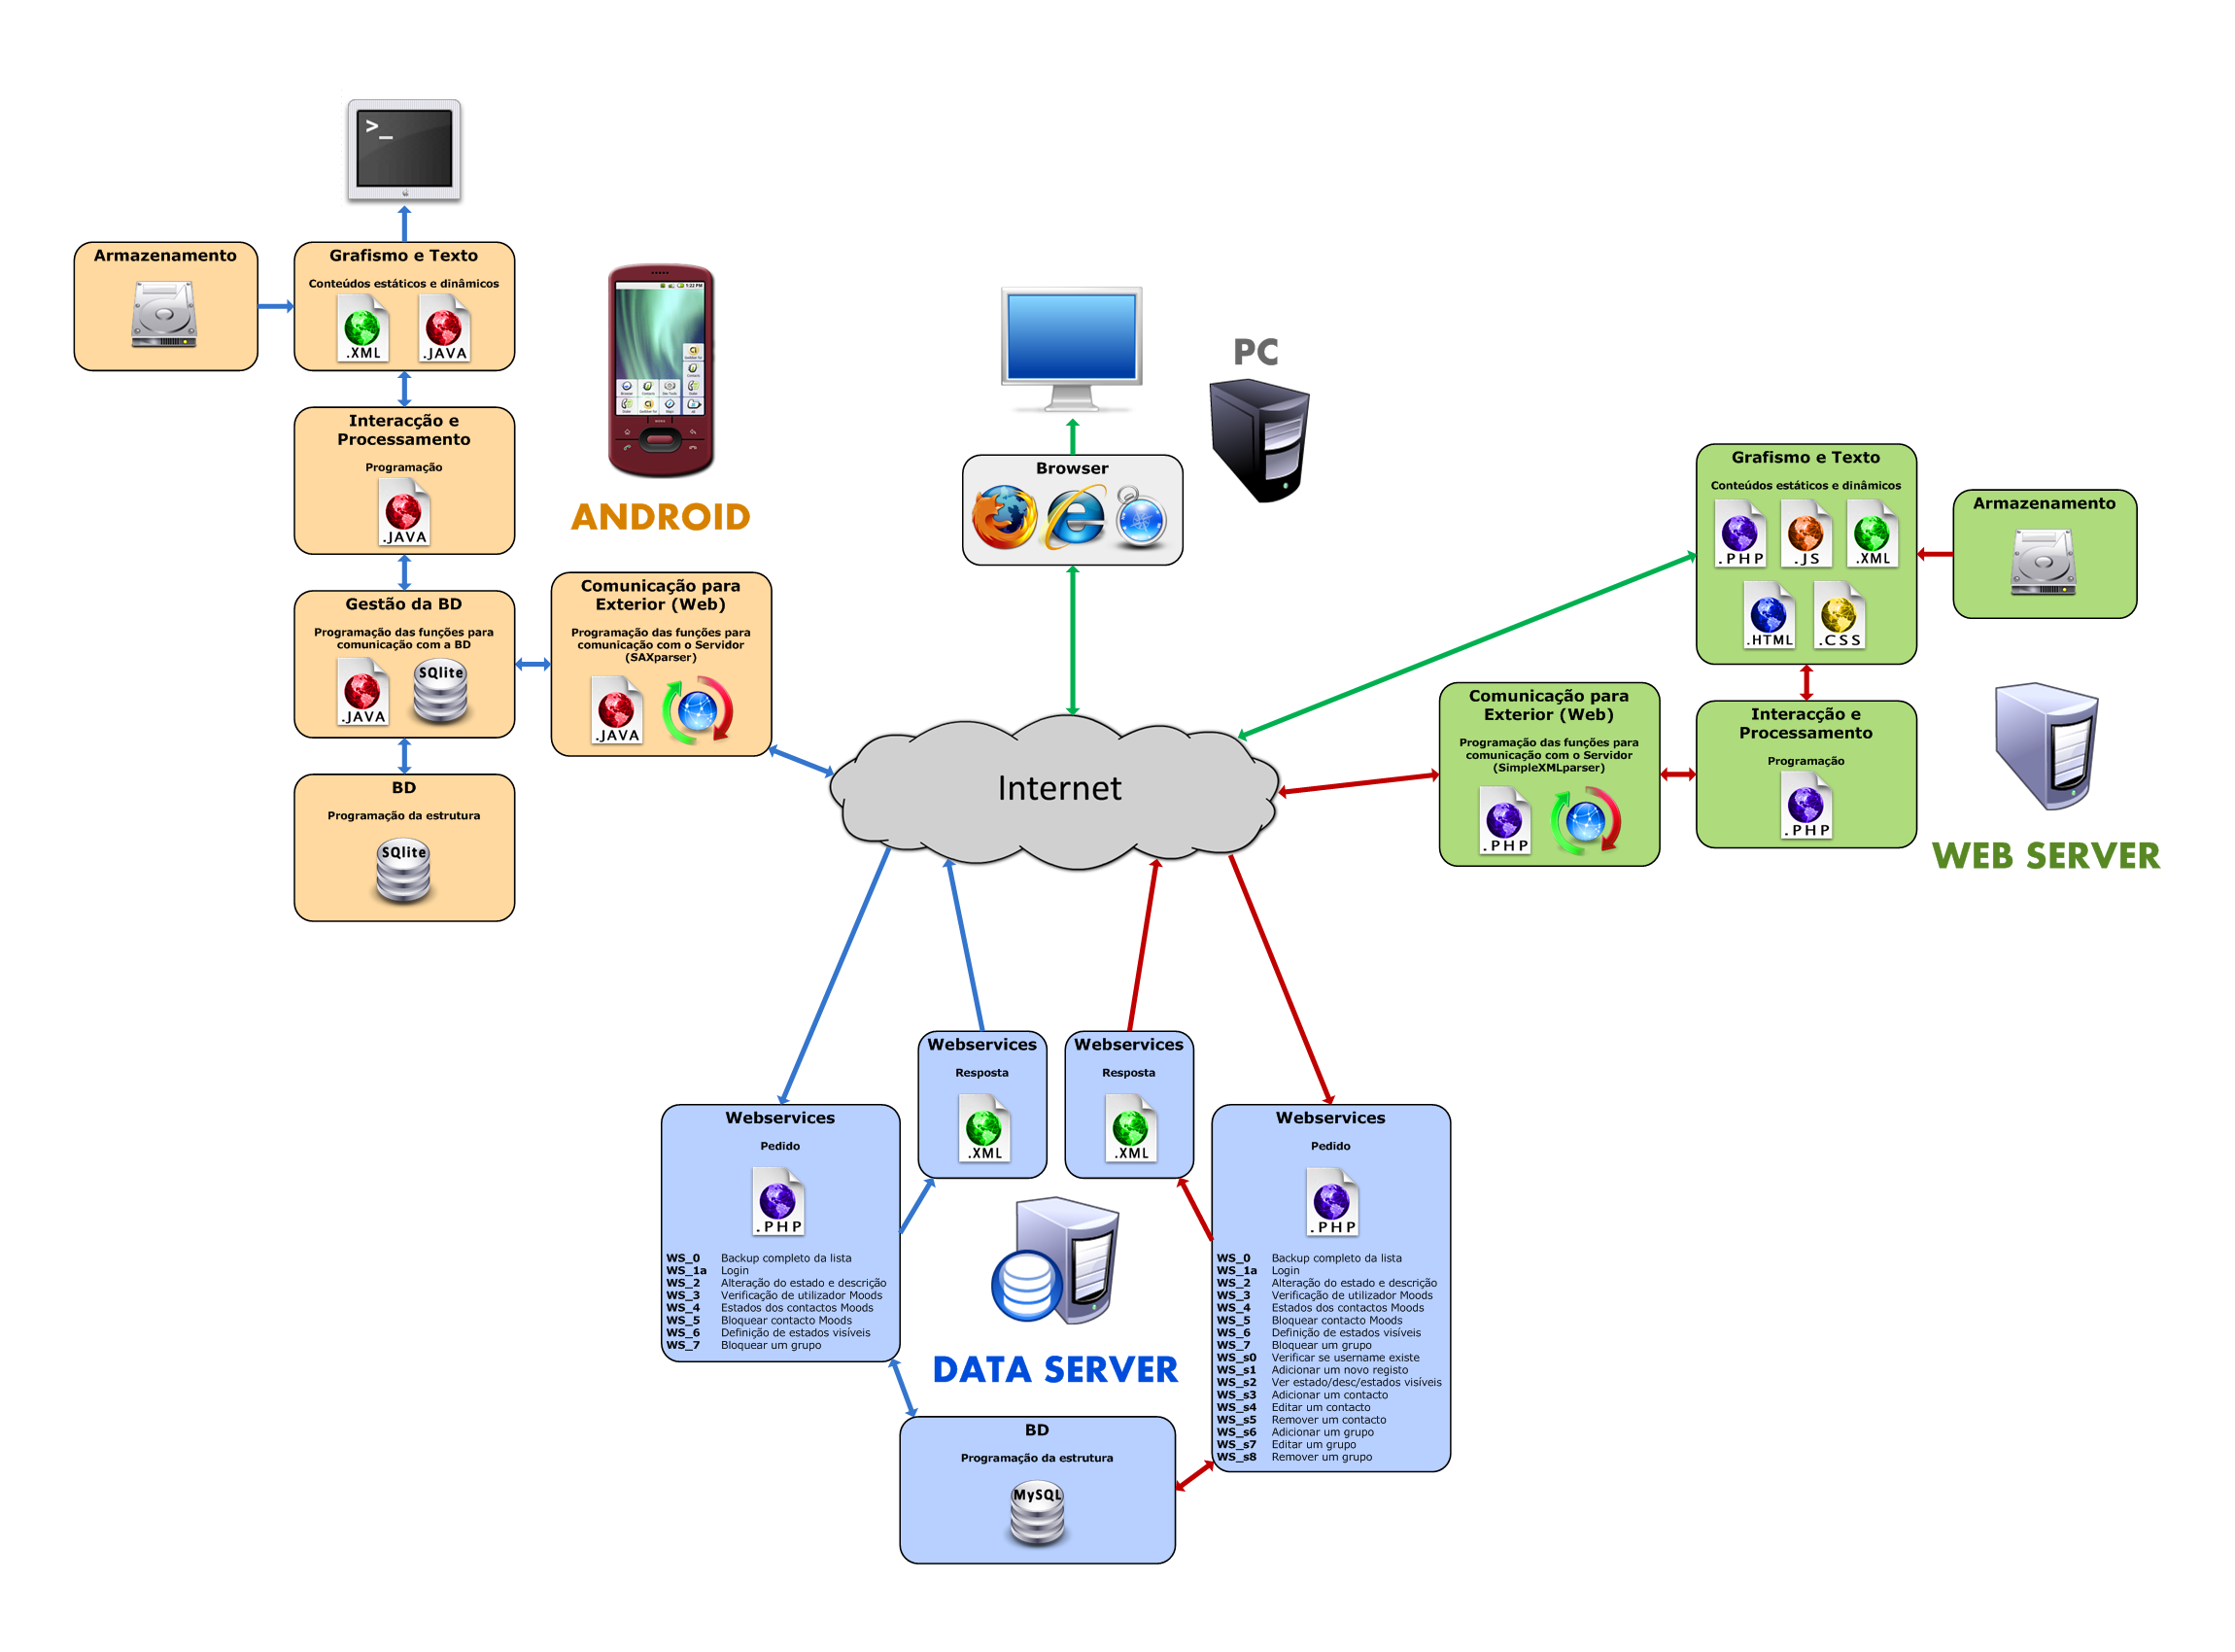
\includegraphics[scale=0.14]{Imagens/webservice.png}
	\caption{Sistema implantando, fornecendo serviços para PCs, dispositivos móveis e outros web servers.}
	\label{wbs}
\end{figure} 

Cada dia existe mais tipos de protocolos porém existem 4 tipo que se destacam: Serviço de Transporte - "FTP", Mensgens "XML", Descrição de Serviço "WSDL"  e Descoberta de Serviço "UDDI".

Podemos observar na figura \ref{wbss}, a pilha de soluções com a pilha de tecnologia correspondente para cada camada. 
\begin{enumerate}
	\item \textbf{Descoberta do serviço:}
	Responsável por centralizar os serviços em um registro comum e fornecer funcionalidades fáceis de publicação/pesquisa. Atualmente, a descoberta do serviço é tratada através de Descrição Universal, Descoberta e Integração (UDDI).
	\item \textbf{Descrição do Serviço:}
	Responsável por descrever a interface pública para um serviço web específico. Atualmente, a descrição do serviço é tratada através do Web Service Description Language (WSDL).
	\item \textbf{Mensagens XML:}
	Responsável por codificar mensagens em um formato XML comum para que as mensagens possam ser entendidas em cada uma das extremidades. Atualmente, esta camada inclui XML-RPC e SOAP.
	\item \textbf{Serviço de transporte:}
	Responsável pelo transporte de mensagens entre aplicativos. Atualmente, esta camada inclui o protocolo de transporte de hipertexto (HTTP), protocolo de transferência de correio simples (SMTP), protocolo de transferência de arquivos (FTP) e protocolos mais recentes, como o protocolo de intercâmbio extensível de blocos (BEEP).
	
	
\end{enumerate}
\begin{figure}[H]
	\centering
	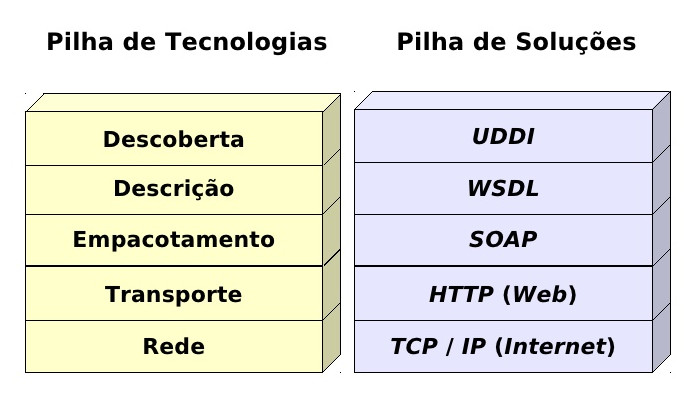
\includegraphics[scale=0.5]{Imagens/pilhat.jpg}
	\caption{Pilha de protocolo de transporte e suas tecnologias. }
	\label{wbss}
\end{figure}


\subsection{Tipos de Web Services}
O mesmo pode ser publicado na intranet ou na Internet, provendo três possiveis formatos de serviços: Provedor de Serviço, Solicitante de Serviço e o Registro de Serviço.
Para mais detalhes desta sessão incentivo a consultar a referência \cite{tutorial}. 

\begin{enumerate}
	\item \textbf{Provedor de serviço:}
	Fornece serviços web. O provedor de serviços implementa o serviço e disponibiliza-o na Internet ou intranet.
	\item \textbf{Solicitante de Serviço:}
	Este é um consumidor do serviço web. O solicitante utiliza um serviço da Web existente abrindo uma conexão de rede e enviando uma solicitação XML.
	\item \textbf{Registro de serviço:}
	Este é um diretório de serviços logicamente centralizado. O registro fornece um lugar central onde os desenvolvedores podem publicar novos serviços ou encontrar os existentes. Ele serve como centro de compensação centralizado para empresas e seus serviços.
\end{enumerate}


\subsection{Componentes de um \textit{Web Service}}
Ao longo dos últimos anos, diversas tecnologias emergiram como padrões mundiais que constituem o núcleo da tecnologia de serviços da Web de hoje. Algumas destas tecnologias e suas caracteristicas são demostradas abaixo.


\subsubsection{WSDL - \textit{Web Services Description Language} }
O WSDL é um idioma baseado em XML, para descrever os serviços da Web e como acessá-los, nas sessões \ref{web:cep} e \ref{web:soap}, será apresentado dois WSDL dos correios, com diversos serviços.

\begin{enumerate}
	\item É um protocolo baseado em XML, para troca de informações em ambientes descentralizados e distribuídos.
	\item É o formato padrão para descrever um serviço web.
	\item Descreve como acessar um serviço da Web e quais as operações que ele executará.
	\item Descrever como se relacionar com serviços baseados em XML.
	\item É o idioma que UDDI utiliza.
	
\end{enumerate}

O WSDL tem um grande papel na arquiteutura de um \textit{Web Service}, ele divulga e expõem os serviços presentes.
\subsubsection{SOAP - \textit{Simple Object Access Protocol}}\label{soapt}

O SOAP é um protocolo baseado em XML para trocar informações entre computadores.

O mesmo não está vinculado a nenhum protocolo de transporte específico. Na verdade, você pode usar SOAP via HTTP, SMTP, FTP ou BEEP.
Algumas caracteriscas estão presentes no SOAP elas são:
\begin{enumerate}
	\item Será desenvolvido como um padrão W3C.
	\item Protocolo de comunicação.
	\item Comunicação entre aplicativos.
	\item Formato para enviar mensagens.
	\item Projetado para se comunicar via Internet.
	\item Independente da plataforma.
	\item Independente da linguagem.
	\item Permite que você percorra os firewalls.
\end{enumerate}
Requisições SOAP serão utilizadas nas sessões \ref{web:cep} e \ref{web:soap}, onde foi utilizado o node-soap uma biblioteca de SOAP para NodeJs.

\subsubsection{REST - \textit{Representation State Transfer}}
É uma arquitetura criada para ser mais simples de se usar que o SOAP. Pode ser usado em vários formatos de texto, como CSV (Comma-separated Values), RSS (Really Simple Syndication), JSON e YAML. Porém, só pode ser utilizado com o protocolo HTTP/HTTPS, por exemplo utilizando os métodos GET, POST, PUT e DELETE. 

\begin{enumerate}
	\item Melhor curva de aprendizado.
	\item Mensagens menores e mais eficientes como o formato JSON comparado com XML.
	\item Os dados podem ser colocados em cache, retornando sempre a mesma resposta para a mesma requisição.
	\item Mais rápido pois precisa de menos processamento que o SOAP.
\end{enumerate}

Como os correios não disponibiliza serviços por REST, foi desenvolvido um serviço alternativo  que será detalhado na sessão \ref{web:alt}.  

\section{\textit{Web Service} - Rafael Buscas }
Nesta sessão relato como foi o desenvolvimento e a implantação de um \textit{Web Service} em um \textit{Web Server}, que promove serviços de busca de CEPs e rastreamento de encomendas dos correios, utilizando uma página web e um aplicativo android como interface para consultas.

\subsection{\textit{Web Server}}
O \textit{Web Server} foi implementado utilizando o NodeJS com o framework ExpressJs, onde se cria um ambiente de desenvolvimento para criação de serviços web.
\begin{quote}
	O Node.js usa um modelo de E/S não bloqueante, que o torna leve e eficiente. O ecossistema de pacotes Node.js, npm , é o maior ecossistema de bibliotecas de código aberto do mundo \cite{nodejs}.
\end{quote}
\begin{quote}
	O Express é um framework para aplicativo da web do Node.js mínimo e flexível que fornece um conjunto robusto de recursos para aplicativos web e móvel \cite{expressjs}.
\end{quote}

\subsection{\textit{Web Service} de Busca de CEP}\label{web:cep}
A busca de cidade e bairro pelo CEP está sendo realiza por um serviço disponível, no WSDL dos 
correios com a url https://apps.correios.com.br/SigepMasterJPA/AtendeClienteService/AtendeCliente?wsdl.

Conforme pode-se observar na figura \ref{c33}, existem diversos serviços neste WSDL, porém só será utilizado o serviço de consulta de cep, com o nome \textit{consultaCEP}.

\begin{figure}[H]
	\centering
	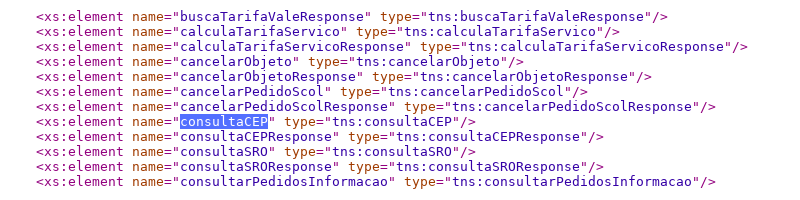
\includegraphics[scale=0.58]{Imagens/wsdlcep.png}
	\caption{Um pedaço dos serviços do WSDL dos correios, com o serviço consultaCEP em azul escuro.}
	\label{c33}
\end{figure}

Utilizando o node-soap (já comentado na sessão \ref{soapt}), uma requisição HTTP-GET de consulta de cep encaminhada para \textit{Web Serve} Rafael Buscas, na url http://rafaelbuscas.ddns.net/api/correios/json/cep/Codigo e recebida por um serviço web, que dispara uma requisição de consulta de cep, por SOAP para o serviço de consulta dos correios, onde após retorno da mesma as informações são repassadas para a requisição inicial.

As linhas de código que recebe a requisição incial, conecta-se ao WSDL dos correios e reenvia a consulta, pode ser objservada na figura \ref{c22}. 

\begin{figure}[H]
	\centering
	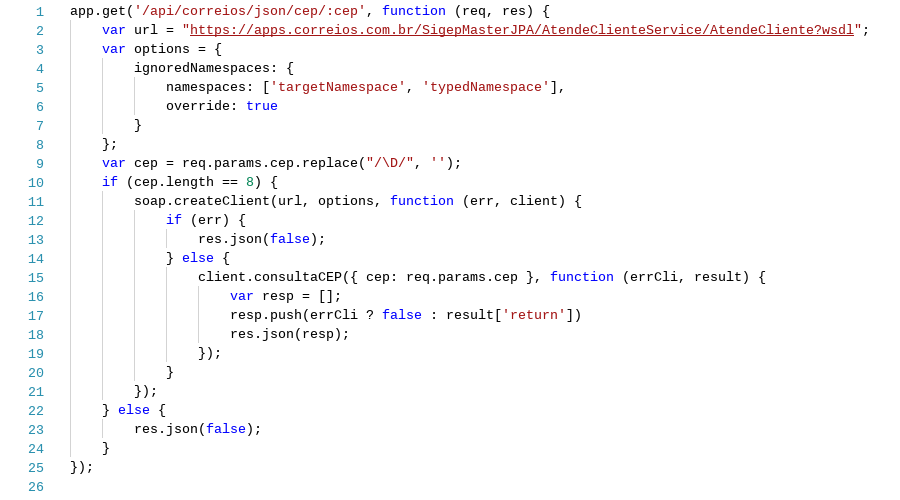
\includegraphics[scale=0.48]{Imagens/codigocep.png}
	\caption{Código de rota, para consulta de cep presente no Web Server Rafael Buscas.}
	\label{c22}
\end{figure}

Para mais informações sobre consulta de cep e outros serviços disponíveis por esse WSDL consultar a referência \cite{correiosapp}.

\subsection{Web Service para rastreamento de encomendas dos Correios}
O rastreamento por encomendas dos correios, desenvolvido nesta sessão, dispõe de duas tecnologias diferentes de empacotamento.

A primeira utiliza a tecnologia SOAP e será apresentada na sessão \ref{web:soap} , a segunda funcional porém alternativa utiliza uma requisição REST HTTP-POST, para obter uma requisição da página oficial dos correios, após receber a resposta em um objeto HTML, é realizado um parsear na resposta para extrair os dados da encomenda, está forma de rastreamento será apresentada na sessão \ref{web:alt}.
\subsubsection{Serviço de Rastreamento Encomenda via SOAP}\label{web:soap}
O WSDL dos correios que fornece o serviço de rastreamento de encomenda conhecido como BuscaEventos, demostrado na figura \ref{wsdl:1}, está disponível na url http://webservice.correios.com.br/service/rastro/Rastro.wsdl.
\begin{figure}[H]
	\centering
	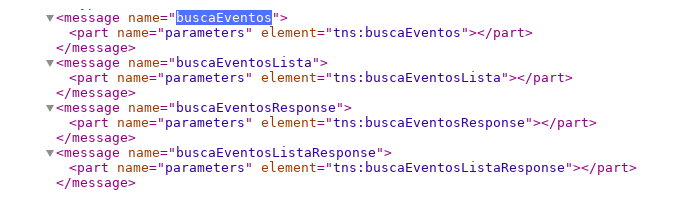
\includegraphics[scale=0.6]{Imagens/wsdlr1.png}
	\caption{Um pedaço dos serviços do WSDL de rastreamento de encomendas dos correios, com o serviço BuscaEventos em azul escuro.}
	\label{wsdl:1}
\end{figure}

Na figura \ref{en:1} utilizando o NodeJS ea biblioteca node-soap, uma solicitação para o \textit{Web Servece} Rafael Buscas com a url http://rafaelbuscas.ddns.net/api/correios/json/objeto/CodigoDoRastreamento, cria uma requisição SOAP, que essa é enviada para o \textit{Web Service} de rastreamento de encomendas, fornecido pelos correios, que retorna uma mesagem JSON que posteriormente e repassada para requisição incial.


Para mais informações referente a API de serviços dos correios, incentivo consultar a referência \cite{correios}.
\begin{figure}[H]
	\centering
	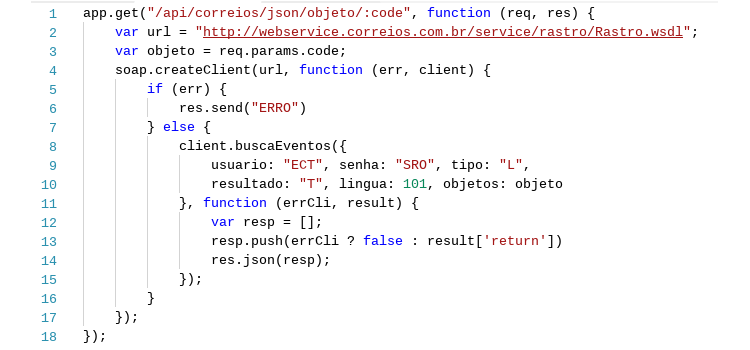
\includegraphics[scale=0.6]{Imagens/codigor1.png}
	\caption{Código de rota, para consulta de encomendas presente no Web Server Rafael Buscas.}
	\label{en:1}
\end{figure}

Esse serviço disponibilizado pelos correios apesar de ser gratuito, somente retorna a última atualização do objeto.
\subsubsection{Serviço de Rastreamento de Encomendas alternativo utilizando Crawling na Página dos Correios}\label{web:alt}

Existe um serviço disponível na página dos correios para rastreamento de encomendas, onde é possivel realizar um crawling na página, para obter um objetivo HTML, contendo as informações da encomenda buscada.

O serviço está disponível na url "http://www2.correios.com.br/sistemas/rastreamento/", a imagem \ref{c1} demostra como pode-se utilizar a ferramenta \textit{Postman}, para realizar uma requisição REST HTTP-POST, direto para página de rastreamento, com objetivo de extrair informações da mesma.

\begin{figure}[H]
	\centering
	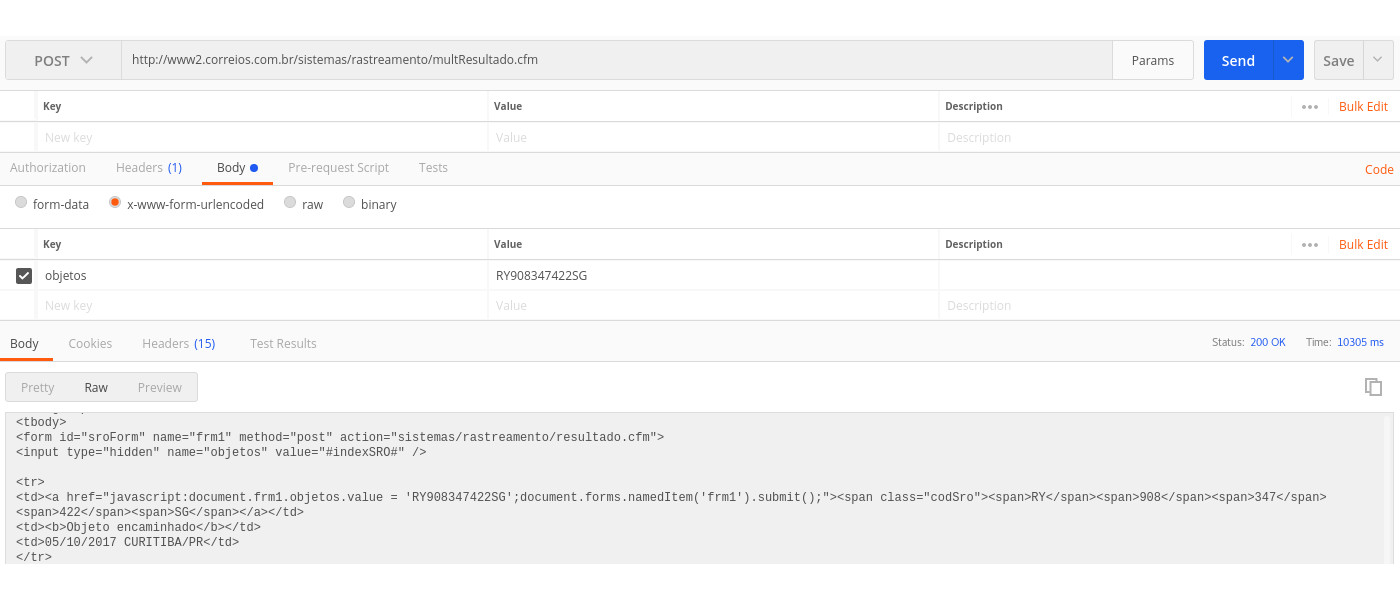
\includegraphics[scale=0.3]{Imagens/c1.jpg}
	\caption{Postman realizando um requsição REST HTTP-POST.}
	\label{c1}
\end{figure}


Para consumir o serviço da página dos correios, primeiramente, foi desenvolvivdo um \textit{Web Service} com NodeJs e o framework ExpressJs, junto com a biblioteca request-promise para requisição JavaScript e a biblioteca cheerio para realizar o parse das tags "tr'' e ''td'' (onde estão as informações da encomenda, demostrado na figura  \ref{c1}, no campo body do response) do HTML.

Na figura \ref{c3} consta um método que realiza uma requisição REST - HTTP-POST no \textit{Web Server} da página web dos correios.
\begin{figure}[H]
	\centering
	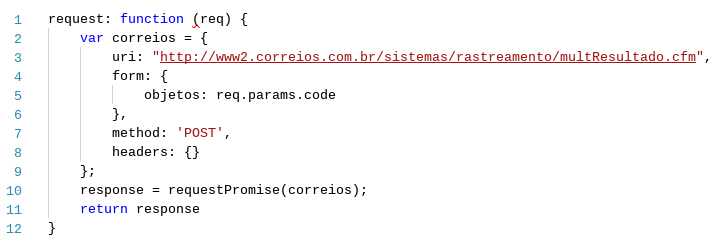
\includegraphics[scale=0.55]{Imagens/req.png}
	\caption{Criando Requisição em Java Script.}
	\label{c3}
\end{figure}

Após a requisição da figura \ref{c3}, teremos uma variável contendo todo o HTML da página web, que foi obtida pela requsição.

Utilizando a função da figura \ref{c4}, realizamos um parse no HTML, com o objetivo de extrair as informações referente a encomenda.

O parse percorre a tabela e extrai, algumas informações (código, localidade, data, situação) criando um objeto JSON, com as informações de rastreamento obtidas, que será consumido pela página web RafaelBuscas.

Assim sendo, uma requisição através da página RafaelBuscas ou utilizando diretamente a url http://rafaelbuscas.ddns.bet/api/correios/json/aobjeto/"codigo-de-rastreamento", primeiramente a requisição é recebida pelo \textit{Web Service} (que está aguardando na rota da url acima), onde o mesmo envia uma requisição HTTP-POST, para a página de rastreamento dos correios com o código de encomenda fornecido, após o parse realizado as informações são encaminhandas em um objeto JSON, como resposta para requisição inicial.   


\begin{figure}[H]
	\centering
	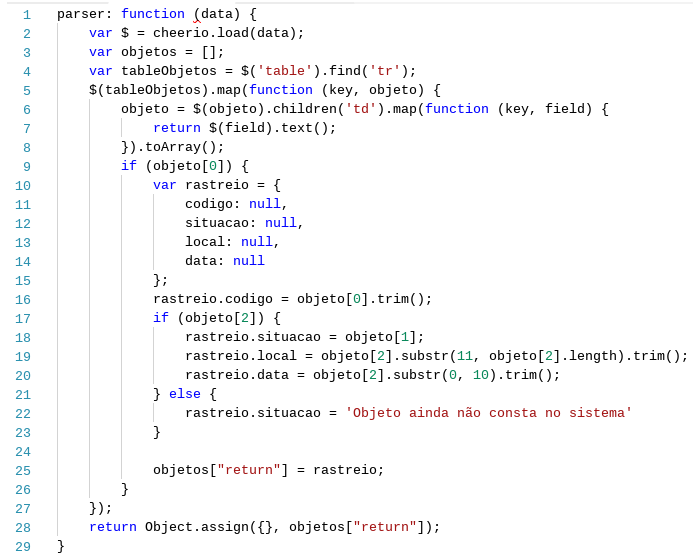
\includegraphics[scale=0.6]{Imagens/par1.png}
	\caption{Criando um Crawling para parsear as tags do HTML.}
	\label{c4}
\end{figure}



\section{Página Rafael Buscas e Aplicativo Android Rafael Buscas}
Para fins didaticos, os serviços de rastreamento de encomendas e buscas de cep pelo código, relatados estão disponíveis na url http://rafaelbuscas.ddns.net, a mesma possui uma página web como interface para os serviços, estes que estão hospedados em uma máquina virtual do Google Cloud.

Na página inical no canto inferior, existe um input para o código do CEP ou do Rastreamento (fornecidos pelos correios).

Um componente para seleção de consulta entre Cep ou Rastremamento, com o nome de ''TIPO'', deve ser marcado como CEP, Rastreio REST ou Rastreio SOAP, antes da busca (botão com uma lupa) como demostrado na Figura \ref{c2}.

\begin{figure}[H]
	\centering
	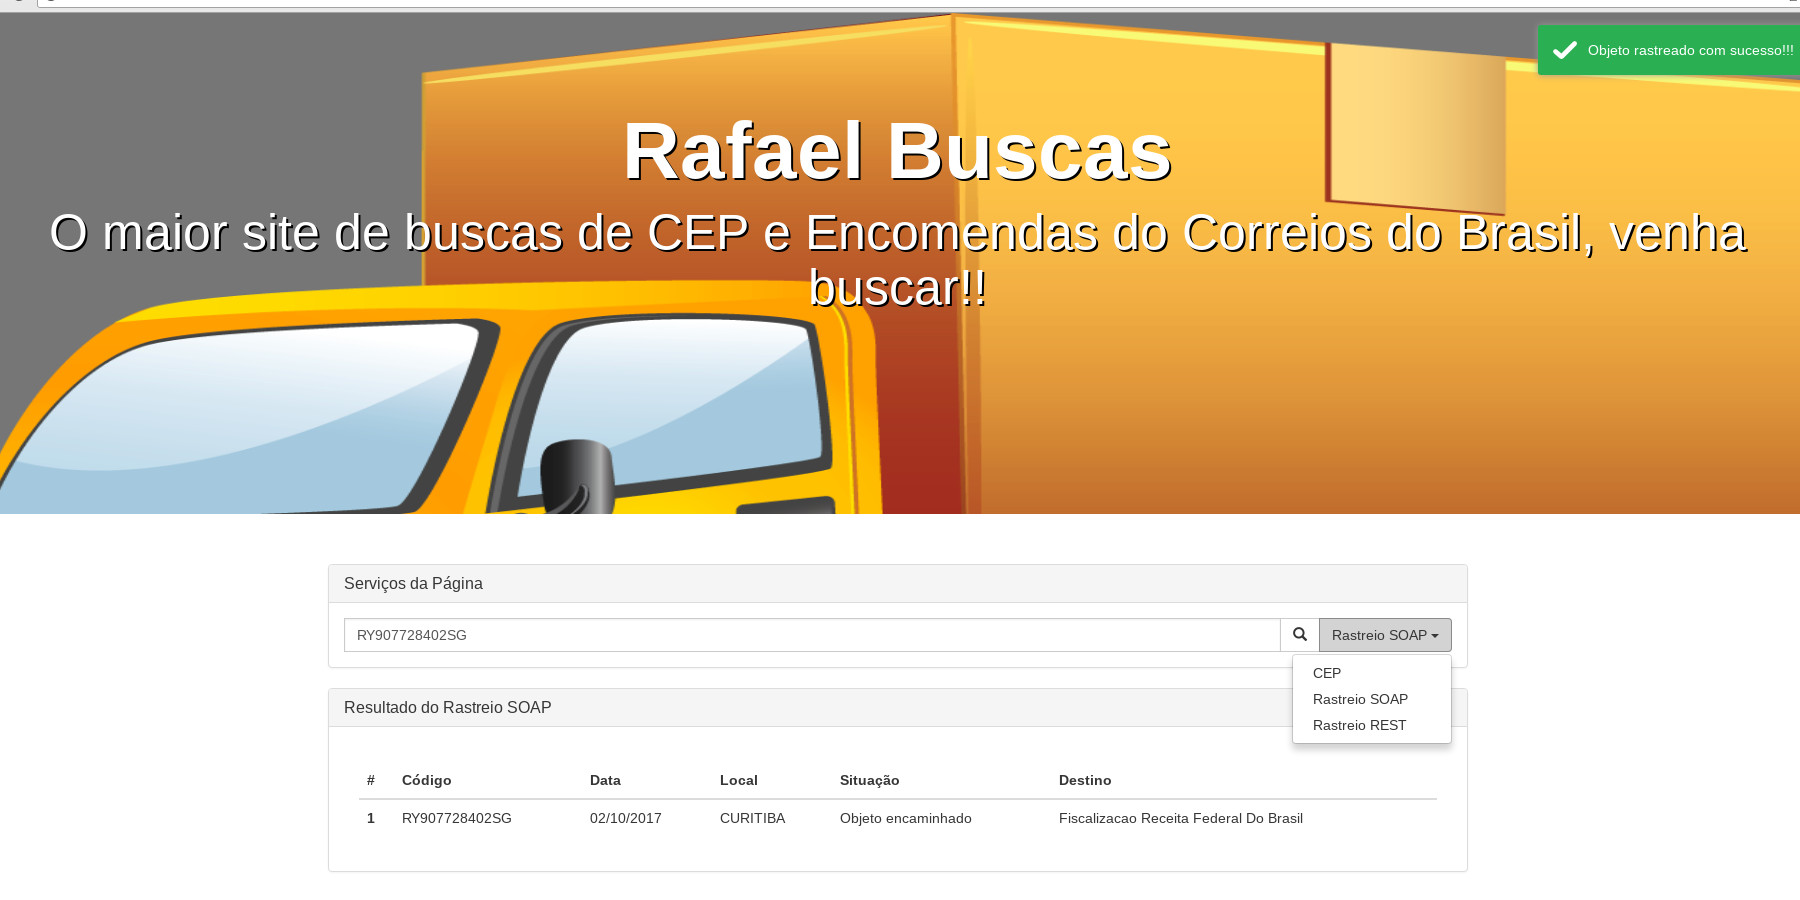
\includegraphics[scale=0.23]{Imagens/c2.jpg}
	\caption{Página Web Rafael Buscas, demostração de busca de encomendas via SOAP.}
	\label{c2}
\end{figure}

Além da página web, um aplicativo para plataforma Android (figura \ref{and}), foi desenvolvido pra demostração de portabilidade dos serviços desenvolvidos neste documento, o mesmo possui as mesmas funcionalidades da página web.

\begin{figure}[H]
	\centering
	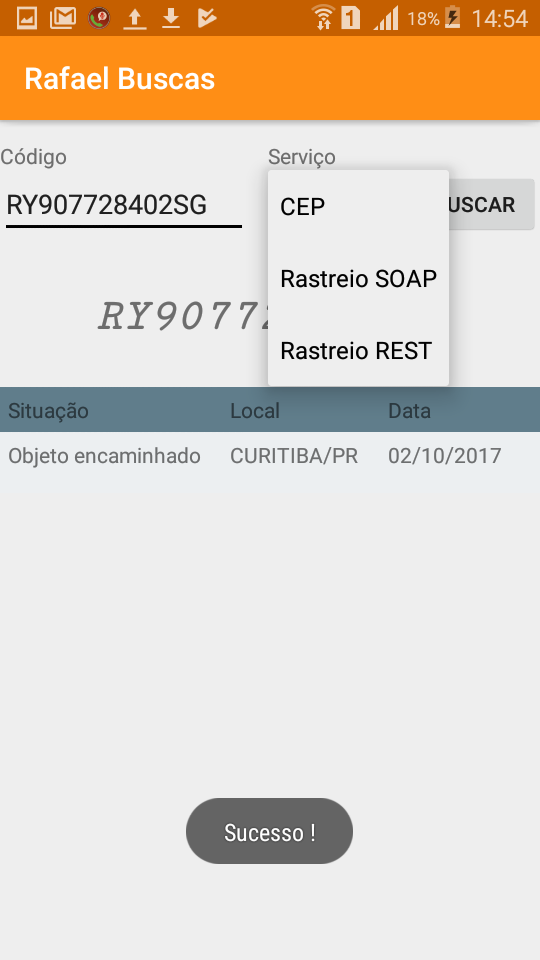
\includegraphics[scale=0.2]{Imagens/android.png}
	\caption{Aplicativo Android Rafael Buscas, demostração de busca de encomendas via SOAP.}
	\label{and}
\end{figure}

\section{Conclusão}
Neste relatório foi apresentado a estrutura básica de um \textit{Web Service}, e como o pŕoprio pode ser utilizado para consumir serviços de outros \textit{Web Services} disponíveis por outras empresas, outra abordagem exposta seria utilizar os mesmos para criação de um novo serviço, em seu próprio \textit{Web Server}, para atender as mais diversas necessidades, como exemplo o rastreiamento de encomendas ou obter a cidade e o bairro através de um CEP.	  	

\bibliography{bibli}

\end{document}


